%%%%%%%% NeurIPS 2025 STYLE %%%%%%%%%%%%%%%%%

\documentclass{article}

\usepackage[preprint]{neurips_2025}

\usepackage[utf8]{inputenc}
\usepackage[T1]{fontenc}
\usepackage{hyperref}
\usepackage{url}
\usepackage{booktabs}
\usepackage{amsfonts}
\usepackage{nicefrac}
\usepackage{microtype}

% Recommended, but optional, packages for figures and better typesetting:
\usepackage{graphicx}
\usepackage{subcaption}

% Attempt to make hyperref and algorithmic work together better:
\newcommand{\theHalgorithm}{\arabic{algorithm}}

\usepackage{amsmath}
\usepackage{amssymb}
\usepackage{mathtools}
\usepackage{amsthm}
\usepackage[capitalize,noabbrev]{cleveref}
\usepackage{xcolor}
\usepackage{multirow}
\usepackage{balance}
\usepackage[ruled,vlined]{algorithm2e}
\crefname{algocf}{Algorithm}{Algorithms}
\Crefname{algocf}{Algorithm}{Algorithms}

% Avoid stretched vertical whitespace in two-column layout.
\raggedbottom

\title{The Shape of Wisdom}
\author{%
  \textbf{Shailesh Rana} \\
  Independent Researcher \\
  \And
  \textbf{Claude Opus 4.6} \\
  \And
  \textbf{ChatGPT Prism} \\
}

\makeatletter
\renewcommand{\@notice}{}
\makeatother

\begin{document}

\twocolumn[
\begin{@twocolumnfalse}
\maketitle

%% ============================================================
%% ABSTRACT
%% ============================================================
\begin{abstract}
We introduce three quantities---\emph{state}, \emph{motion}, and \emph{boundary}---that fully describe the layer-by-layer trajectory of a transformer's answer on multiple-choice benchmarks.
The \textbf{state} is the logit margin between the model's preferred answer and its strongest competitor at each layer.
\textbf{Motion} is the per-layer change in that margin.
\textbf{Boundary} is its absolute magnitude, measuring proximity to a decision flip.
Across three 7--8B instruction-tuned transformers, these primitives separate prompts into four trajectory types---\emph{stable-correct}, \emph{stable-wrong}, \emph{unstable-correct}, and \emph{unstable-wrong}---producing a phase diagram that replicates across models and knowledge domains.
We decompose motion into attention and MLP contributions, defining each as the margin change in logits induced by the respective residual-stream update, and achieve drift reconstruction $R^2 \geq 0.70$ on held-out data.
Linearized counterfactual accounting via simulated component removal, activation substitution, and input-level span-deletion experiments---controlled against shuffled and sign-flipped baselines with Benjamini--Hochberg correction---confirms directionally consistent, finite effects on the decision margin.
\end{abstract}
\vspace{0.2cm}
\end{@twocolumnfalse}
]

%% ============================================================
%% 1. INTRODUCTION
%% ============================================================
\section{Introduction}

A transformer answering a multiple-choice question does not make a single decision.  It makes one decision per layer.  At layer zero the output logits are largely uninformed; by the final layer they commit to an answer.  What happens in between---whether the trajectory converges smoothly, oscillates, or drifts into the wrong basin---determines whether the model answers correctly.

Prior work in mechanistic interpretability has illuminated transformer internals through probing classifiers~\cite{belinkov2022}, causal tracing~\cite{meng2022}, and circuit-level analysis~\cite{olsson2022,conmy2023}.
These approaches identify \emph{what} a model knows and \emph{where} it stores that knowledge, yet typically treat the final output as a binary event rather than examining the dynamic \emph{process} by which the model arrives at it across its full depth.

We propose a complementary perspective.  Rather than asking what a model has learned, we ask: \emph{what does the trajectory of a model's decision look like as it propagates through layers, and can we predict convergence outcomes from a small set of trajectory-level quantities?}

Our answer is yes.  We define three primitives---\textbf{state} (the logit margin~$\delta$), \textbf{motion} (per-layer drift~$g$), and \textbf{boundary} (the absolute margin~$|\delta|$)---and show that they suffice to classify decision trajectories into four outcome types that replicate across models and domains.  We then decompose motion into attention and MLP contributions and assess the resulting mechanistic claims via counterfactual accounting.

\paragraph{Contributions.}
\begin{enumerate}
\item A physics-inspired framework for analyzing transformer decisions as trajectories in logit-margin space, characterized by three measurable quantities.
\item A phase diagram with four well-separated trajectory types, replicated across three architectures and multiple knowledge domains.
\item A linear decomposition of per-layer drift into attention and MLP components with $R^2 \geq 0.70$ on held-out data and a mechanistic interpretation of routing versus injection.
\item Counterfactual accounting experiments---simulated component removal, activation substitution, and input-level span deletion---with multiple-comparison-corrected tests and negative controls.
\end{enumerate}


%% ============================================================
%% 2. THE THREE PRIMITIVES
%% ============================================================
\section{Margin, Drift, and Boundary}
\label{sec:primitives}

We study four-choice (A/B/C/D) questions.  At each transformer layer $l \in \{0,\ldots,L{-}1\}$, we extract logits for the four answer tokens and define all quantities in the restricted four-candidate subspace.

\paragraph{Token-bucket readout.}
Tokenizers map the same letter to different token IDs depending on surrounding context (e.g.\ \texttt{"A"}, \texttt{" A"}, \texttt{"(A)"}, \texttt{"A."}, \texttt{"A:"}, \texttt{"\textbackslash nA"}).
To ensure the readout captures the strongest signal regardless of surface form, we construct a \emph{token bucket} for each answer letter containing the token IDs of six variant templates.
Each template string is normalized via Unicode NFKC, stripped of whitespace, uppercased, and stripped of surrounding punctuation before tokenization.
The score for answer $k$ at layer $l$ is
\begin{equation}
  z_k(l) = \max_{t \,\in\, \mathrm{bucket}(k)} \operatorname{logit}_t(l).
  \label{eq:bucket}
\end{equation}
Bucket disjointness is enforced: if any token ID appears in more than one bucket, the pipeline halts with an error.  All logits, probabilities, and correctness decisions reported in this paper use this \emph{restricted-choice} readout, not full-vocabulary prediction.  Correctness is determined by argmax of $z_k(L{-}1)$ over $k \in \{\mathrm{A}, \mathrm{B}, \mathrm{C}, \mathrm{D}\}$ at the final transformer layer.

\subsection{State: The Decision Margin}

Let $z_c(l)$ denote the bucket score for the correct answer and $z_{k^*}(l)$ the score for the \textbf{closest competitor}---the highest-scoring incorrect option, recomputed at each layer:
\begin{equation}
  k^*(l) = \arg\max_{k \neq c}\; z_k(l).
  \label{eq:competitor}
\end{equation}
The \textbf{decision margin} is:
\begin{equation}
  \delta(l) = z_c(l) - z_{k^*}(l).
  \label{eq:delta}
\end{equation}
When $\delta(l) > 0$ the model favors the correct answer; the sign at the final layer determines correctness.

\emph{Design decision.}  We track competitor identity $k^*(l)$ per layer rather than fixing it globally.  The competitor can change identity across layers.  A sign flip in~$\delta$ can therefore arise from two distinct mechanisms: (i)~\emph{evidence reversal}, where the same competitor overtakes the correct answer, or (ii)~\emph{competitor switch}, where a different option becomes the strongest competitor.  When the competitor switches between layers, the drift $g(l)$ reflects a change in the margin against a different opponent, making it a less direct measure of momentum toward correctness.

\subsection{Motion: Layer-by-Layer Drift}

The \textbf{drift} is the per-layer change in decision margin:
\begin{equation}
  g(l) = \delta(l{+}1) - \delta(l),
  \label{eq:drift}
\end{equation}
with $g(L{-}1) \equiv 0$.  Positive drift moves toward the correct answer.

\subsection{Boundary Proximity}

The \textbf{boundary distance} is the unsigned state:
\begin{equation}
  b(l) = |\delta(l)|.
  \label{eq:boundary}
\end{equation}
Small $b$ means proximity to a decision flip.

\subsection{Convergence and Trajectory Types}

A trajectory is \textbf{stable} if, within a tail window of the last $\tau$ layers, $\delta(l)$ maintains a consistent sign and $b(l) \geq b_{\min}$ throughout.  Combined with final-layer correctness this yields four types: \emph{stable-correct}, \emph{stable-wrong}, \emph{unstable-correct}, \emph{unstable-wrong}.

We use $\tau = 8$, require zero sign flips, and enforce $b_{\min} = 0.3$.  These thresholds were pre-registered.  Sensitivity analysis appears in \cref{sec:appendix_sensitivity}.


\begin{figure*}[t]
  \vskip 0.1in
  \begin{center}
    \centerline{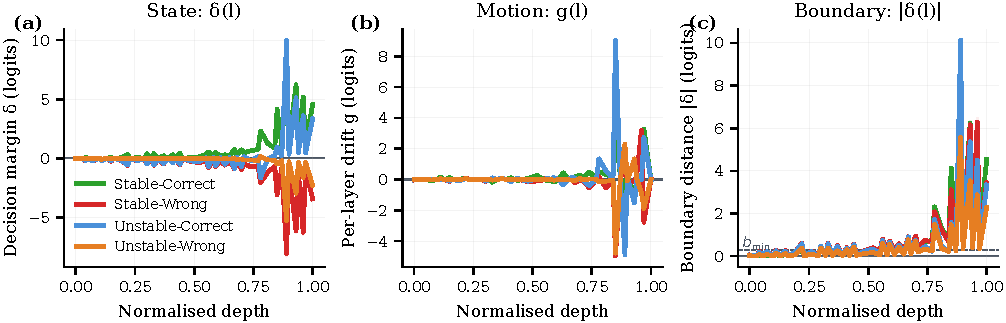
\includegraphics[width=0.95\textwidth]{figures/fig1_primitives.pdf}}
    \caption{The three primitives averaged across all three models with layer depth normalized to $[0,1]$.
    \textbf{(a)}~Mean decision margin $\delta$ (logits) by trajectory type; shaded bands show $\pm$\,SEM for stable types.
    \textbf{(b)}~Mean per-layer drift $g$ (logits).
    \textbf{(c)}~Mean boundary distance $|\delta|$ (logits); dashed line marks $b_{\min} = 0.3$.
    Data: \texttt{decision\_metrics.parquet} (276{,}000 rows), \texttt{prompt\_types.parquet} (9{,}000 rows).
    Lines: 4 trajectory types.  $x$-axis: normalised depth $l/(L{-}1)$.}
    \label{fig:primitives}
  \end{center}
\end{figure*}


%% ============================================================
%% 3. EXPERIMENTAL SETTING
%% ============================================================
\section{Experimental Setup}
\label{sec:experiments}

\subsection{Models}

We study three instruction-tuned transformers spanning distinct pre-training recipes at controlled scale (\cref{tab:models}).  All are loaded at pinned HuggingFace revisions with deterministic decoding (temperature~$= 0$, \texttt{do\_sample=false}, seed~$= 12345$).  Left-padding with explicit position IDs is enforced for batched inference.

\begin{table}[t]
  \caption{Models used in this study, with pinned revisions.}
  \label{tab:models}
  \vskip 0.1in
  \begin{center}
  \begin{small}
  \begin{sc}
  \begin{tabular}{lcc}
    \toprule
    Model & Params & Layers \\
    \midrule
    Qwen 2.5-7B-Instruct  & 7.6B & 28 \\
    Llama 3.1-8B-Instruct  & 8.0B & 32 \\
    Mistral 7B-v0.3 & 7.2B & 32 \\
    \bottomrule
  \end{tabular}
  \end{sc}
  \end{small}
  \end{center}
\end{table}

\subsection{Data}

We draw 3{,}000 four-choice questions from MMLU~\cite{hendrycks2021}, balanced across difficulty levels and knowledge domains.  The manifest is SHA-256 hashed and version-locked before inference.

\subsection{Logged Quantities}

For each prompt~$\times$~model pair we record layerwise logits, probabilities, and entropy for the four candidate token buckets at every \emph{transformer} layer (embedding layers excluded).

For a tracing subset (600 prompts per model, balanced over trajectory type and difficulty), we additionally capture per-layer attention outputs, MLP outputs, and attention weight matrices via forward hooks with eager attention.

\subsection{Why Logit Space?}

$\delta$, $g$, and $b$ are computed directly from token-bucket logits; trajectory type is a deterministic function of these.  The attention/MLP decomposition involves a linear fit, and counterfactual experiments use both linearized drift bookkeeping and input-level span deletion.  We maintain this distinction throughout.

Softmax probabilities compress high-confidence decisions into a near-saturated regime.  Logit margins preserve ordinality and scale.  Probability-space analyses appear in \cref{sec:appendix_prob}.


%% ============================================================
%% 4. PHASE DIAGRAM
%% ============================================================
\section{Trajectory Classification}
\label{sec:phase}

\subsection{Four Trajectory Outcomes}

Each prompt~$\times$~model pair is classified into exactly one of four types (\cref{tab:types}).

\begin{table}[t]
  \caption{The four trajectory types.}
  \label{tab:types}
  \vskip 0.1in
  \begin{center}
  \begin{small}
  \resizebox{\columnwidth}{!}{%
  \begin{tabular}{lccl}
    \toprule
    Type & Corr. & Stab. & Interpretation \\
    \midrule
    Stable-corr.   & \checkmark & \checkmark & Knew, stayed confident \\
    Stable-wrong   & $\times$   & \checkmark & Committed to wrong ans. \\
    Unstable-corr. & \checkmark & $\times$ & Oscillated, landed right \\
    Unstable-wrong & $\times$   & $\times$ & Oscillated and failed \\
    \bottomrule
  \end{tabular}%
  }
  \end{small}
  \end{center}
\end{table}

\subsection{Phase Structure}

We plot boundary proximity at tail entry $|\delta(L{-}\tau)|$ against the number of sign flips of $\delta$ in the last $\tau = 8$ layers (\cref{fig:phase}).  These two axes are algebraically independent---unlike the pair $(\delta(L),\, \Sigma g)$ where $\Sigma g$ telescopes to $\delta(L) - \delta(L{-}\tau)$, creating partial redundancy.

Stable types cluster at high boundary proximity and zero tail flips; unstable types populate the higher-flip region with lower boundary values.

\begin{figure}[t]
  \vskip 0.1in
  \begin{center}
    \centerline{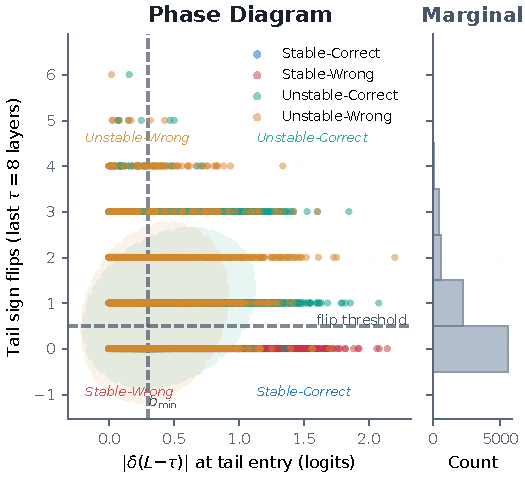
\includegraphics[width=\columnwidth]{figures/fig2_phase_diagram.pdf}}
    \caption{Phase diagram with non-redundant axes.  $x$-axis: boundary proximity at tail entry $|\delta(L{-}\tau)|$ (logits); $y$-axis: number of sign flips in the last $\tau = 8$ layers; jittered $\pm 0.10$.  Each point is one prompt~$\times$~model pair ($N = 9{,}000$).  Dashed lines: $b_{\min} = 0.3$ (vertical), flip threshold $= 0.5$ (horizontal).
    Data: \texttt{decision\_metrics.parquet}, \texttt{prompt\_types.parquet}.}
    \label{fig:phase}
  \end{center}
\end{figure}


\subsection{Cross-Model and Cross-Domain Replication}

The phase structure replicates qualitatively across all three models.  Absolute magnitudes differ---Qwen produces larger $|\delta|$ than Mistral---but the four-region geometry and the separation between stable and unstable types are consistent.  Domain shifts the \emph{proportion} of types but not the geometry.

\emph{Caveat.}  The clean separation partly reflects our threshold choices.  Clusters remain visually distinct under perturbations ($\tau \in \{6, 8, 10\}$, $b_{\min} \in \{0.1, 0.3, 0.5\}$), but the boundary between stable and unstable is a convention, not a natural discontinuity.  We adopt \emph{phase diagram} as a visual metaphor for a classification map.  Stability boundaries depend on threshold conventions ($\tau$, $b_{\min}$, flip count) and shift smoothly under perturbation.


%% ============================================================
%% 5. TWO-FORCE DECOMPOSITION
%% ============================================================
\section{Drift Decomposition}
\label{sec:decomposition}

\subsection{Component Scalars as Margin Change}

At each layer~$l$, the residual stream update sums two components: the attention sub-layer output~$a(l)$ and the MLP sub-layer output~$m(l)$.  Denoting the residual stream before the sub-layers as $h_{\mathrm{in}}(l)$, the post-attention state is $h_{\mathrm{in}} + a$ and the post-MLP state is $h_{\mathrm{in}} + a + m$.

We define the \textbf{attention scalar} and \textbf{MLP scalar} as the change in decision margin caused by each update:
\begin{align}
  s_{\mathrm{attn}}(l) &= \delta(h_{\mathrm{in}} + a) - \delta(h_{\mathrm{in}}), \label{eq:s_attn} \\
  s_{\mathrm{mlp}}(l) &= \delta(h_{\mathrm{in}} + a + m) - \delta(h_{\mathrm{in}} + a), \label{eq:s_mlp}
\end{align}
where $\delta(h)$ denotes applying the unembedding matrix $W_U$ to the hidden state~$h$ and computing the correct-minus-competitor margin among token-bucket scores.
In the tracing pipeline, this margin is read out from canonical single-token option labels (\texttt{A}/\texttt{B}/\texttt{C}/\texttt{D}) to match stored tracing artifacts.
Baseline trajectory metrics elsewhere in the paper use token-bucket scoring (\cref{eq:bucket}), so decomposition scalars are a tracing-specific linear proxy under the same per-layer competitor rule.

\paragraph{Equivalence to a dot product.}
Because $\delta(h) = h^\top W_U^\top (e_c - e_{k^*})$ and $W_U$ is a linear operator,
\begin{equation}
  s_{\mathrm{attn}}(l) = a(l)^\top W_U^\top\, d(l),
  \label{eq:attn_dot}
\end{equation}
where $d(l) = e_c - e_{k^*(l)}$ is the \textbf{decision direction} at layer~$l$.  The scalar is therefore a signed quantity in logit-margin units: positive means the component pushed toward the correct answer, negative means it pushed away.  It is \emph{not} an angle or a cosine similarity.  The same derivation applies to $s_{\mathrm{mlp}}$.

\subsection{Drift Reconstruction}

Observed drift should be approximated by:
\begin{equation}
  g(l) \approx \alpha \cdot s_{\mathrm{attn}}(l) + \beta \cdot s_{\mathrm{mlp}}(l) + \varepsilon.
  \label{eq:decomposition}
\end{equation}
We fit via OLS on a 70/30 train/test split (at the prompt level).  The pipeline requires $R^2 \geq 0.70$ on test data; this gate was pre-registered.

\emph{Why linear?}  A richer model would fit better but explain less.  The residual $\varepsilon$ captures layer-norm effects, cross-term dependencies, and nonlinear interactions.

\subsection{What Each Component Does}

\cref{fig:decomposition} reveals the following patterns:

\textbf{Attention is the dominant positive force early and mid-depth.}  In stable-correct trajectories (\cref{fig:decomposition}a), $s_{\mathrm{attn}}$ is broadly positive through the central depth range and tracks positive observed drift.

\textbf{MLP contribution is context-dependent and often late-weighted.}  In stable-correct trajectories, MLP contributes a short late positive burst while remaining mixed elsewhere; in stable-wrong trajectories, both components are frequently negative and reinforce wrong commitment (\cref{fig:decomposition}b).

\textbf{Dominance depends on the diagnostic.}  Using positive-steering share, attention contributes most early positive shifts while MLP contributes most late positive shifts (\cref{fig:decomposition}c).  Sign-alignment and oscillation diagnostics vary by trajectory type but do not yield a single clean separating threshold (\cref{fig:decomposition}d,e).


\begin{figure*}[t]
  \vskip 0.1in
  \begin{center}
    \centerline{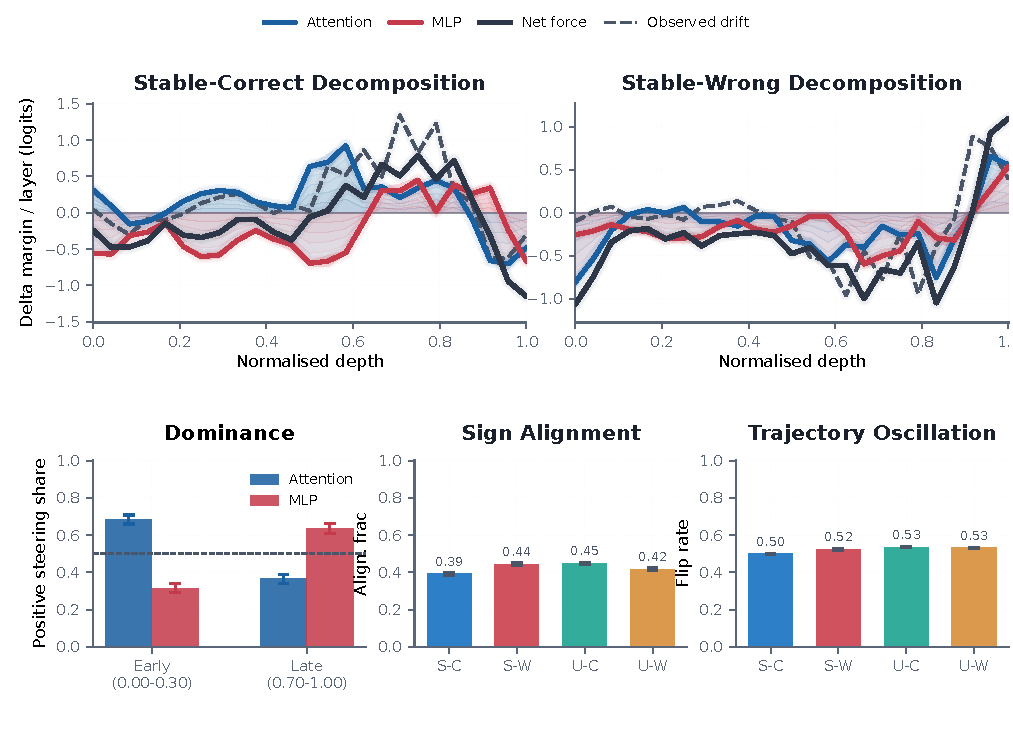
\includegraphics[width=\textwidth]{figures/fig3_decomposition.pdf}}
    \caption{Drift decomposition and diagnostics from stored traces.
    \textbf{(a,b)}~Mean component traces for stable-correct and stable-wrong with SEM bands, plus observed drift $g$ (all in logit-margin units per layer).
    \textbf{(c)}~Early-vs-late positive-steering dominance (attention share vs.\ MLP share) with bootstrap 95\% CI.
    \textbf{(d)}~Fraction of layers where attention and MLP contributions share sign.
    \textbf{(e)}~Oscillation proxy (drift sign-change rate).
    Data: \texttt{tracing\_scalars.parquet} (55{,}200 rows), \texttt{decision\_metrics.parquet}, \texttt{prompt\_types.parquet}.}
    \label{fig:decomposition}
  \end{center}
\end{figure*}


%% ============================================================
%% 6. ATTENTION AS ROUTING
%% ============================================================
\section{Attention and Span Routing}
\label{sec:routing}

\subsection{Prompt Span Taxonomy}

Multiple-choice prompts have natural structure: \emph{instruction}, \emph{question stem}, and \emph{option spans} (A--D).  We parse these via regex-based boundary detection.  For analysis, option spans are re-indexed \emph{relative to correctness}: \texttt{option\_correct} (the ground-truth answer), \texttt{option\_competitor} (the strongest wrong option at the final layer), and \texttt{option\_other} (remaining wrong options, averaged).

\subsection{Span Labeling: An Operational Definition}

We \emph{define} evidence and distractor spans operationally via counterfactual deletion.  For each span $s$, we delete it from the prompt and re-run inference.  The margin-change effect is:
\begin{equation}
  \Delta(s) = \delta_{\mathrm{full}} - \delta_{\mathrm{deleted}}.
  \label{eq:span_effect}
\end{equation}
Spans with $\Delta \geq 0.05$ are labeled \emph{evidence}; $\Delta \leq -0.05$ are \emph{distractor}; otherwise \emph{neutral}.

\emph{This labeling is an operational definition, not a discovery.}  By construction, evidence spans have positive $\Delta$ and distractor spans have negative $\Delta$.  Their separation by $\Delta$ magnitude is therefore tautological.  The value of these labels lies in enabling downstream analyses where we can ask: do attention routing patterns, decision-aligned contributions, and negative controls independently corroborate the functional distinction?

\textbf{Validation via independent signals.}  Three lines of evidence support the labels beyond the circular definition: (i)~attention mass routing shows disproportionate weight toward evidence-labeled spans in stable-correct trajectories (\cref{fig:routing}a); (ii)~decision-aligned contribution mirrors this pattern (\cref{fig:routing}b); (iii)~negative controls (shuffled and sign-flipped baselines) center at zero while observed evidence-labeled effects are significantly larger (\cref{fig:causal}d).

Label stability under paraphrase: $\geq 85\%$ agreement, $\geq 0.80$ Jaccard similarity.

\subsection{Attention Mass vs.\ Contribution}

We distinguish \textbf{attention mass} (raw weight from answer position to span tokens, normalized per token) from \textbf{decision-aligned contribution} (the attention output projected onto $d$, per \cref{eq:attn_dot}).

\cref{fig:routing} presents routing in two complementary views.  The stacked-mass panels (\cref{fig:routing}a,b) show how span-role allocation evolves with depth for stable-correct versus stable-wrong trajectories.  The contribution heatmap (\cref{fig:routing}c) shows that decision-aligned attention on \texttt{option\_correct} is strongest for stable-correct trajectories, while stable-wrong trajectories shift contribution toward competitor-aligned structure.

\begin{figure*}[t]
  \vskip 0.1in
  \begin{center}
    \centerline{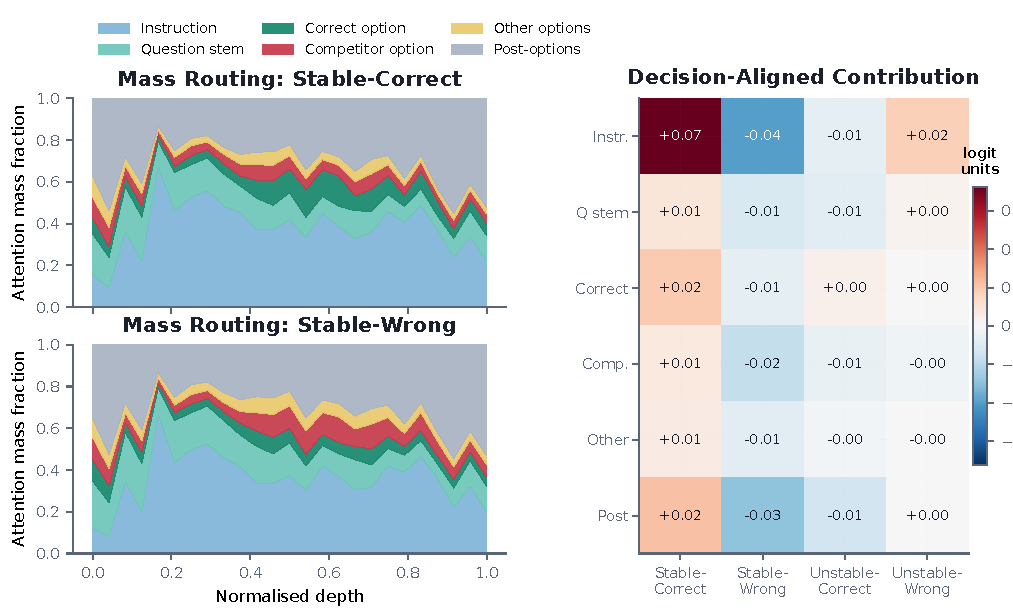
\includegraphics[width=\textwidth]{figures/fig4_attention_routing.pdf}}
    \caption{Attention routing by span role.
    \textbf{(a)}~Role-normalized stacked attention mass across depth for stable-correct trajectories.
    \textbf{(b)}~Same stacked-mass view for stable-wrong trajectories.
    \textbf{(c)}~Decision-aligned attention contribution heatmap (mean logit units) by span role and trajectory type; diverging color scale centered at zero.
    Data: \texttt{attention\_mass\_by\_span.parquet} (386{,}400 rows), \texttt{attention\_contrib\_by\_span.parquet} (386{,}400 rows), \texttt{decision\_metrics.parquet}, \texttt{prompt\_types.parquet}.}
    \label{fig:routing}
  \end{center}
\end{figure*}


%% ============================================================
%% 7. MLP AS INJECTION
%% ============================================================
\section{MLP Contributions}
\label{sec:mlp}

The MLP scalar $s_{\mathrm{mlp}}(l)$ measures how much each layer's feedforward network contributes to the decision margin (\cref{eq:s_mlp}).  Unlike attention, MLP can introduce information absent from the input---stored associations, factual recall, and learned biases.

In stable-correct trajectories, MLP shows a brief late supportive phase but is not uniformly positive across depth (\cref{fig:decomposition}a,c).  The practical pattern is not a pure handoff where MLP simply \"takes over\" late; it is a mixed signal whose net effect depends on layer and trajectory context.

For stable-wrong trajectories, both components are net negative---attention routes toward the competitor and MLP reinforces the wrong commitment.  The absence of a corrective force from either component explains why these trajectories are stable in the wrong basin.


%% ============================================================
%% 8. CAUSAL VALIDATION
%% ============================================================
\section{Counterfactual Accounting Experiments}
\label{sec:causal}

Sections~\ref{sec:decomposition}--\ref{sec:mlp} are correlational.  We conduct three families of counterfactual experiments.  The first two (simulated removal and substitution) operate on a \emph{linearized drift-bookkeeping model} rather than full forward-pass interventions; only span deletion involves true input-level interventions with full re-inference.

\subsection{Simulated Component Removal}

We estimate the effect of removing a component by subtracting its scalar from drift at target layers and recomputing the counterfactual final margin.

\emph{Intuition:} if we ``erase'' the attention (or MLP) contribution at selected layers, how much does the final margin shift?  The linearized estimate assumes later layers do not adapt to the modified intermediate state.

\begin{algorithm}[t]
\DontPrintSemicolon
\caption{Simulated Component Removal}\label{alg:removal}
\KwIn{drift $g[0..L{-}1]$, component scalar $s[0..L{-}1]$, target layers $T$, initial margin $\delta_0$}
\KwOut{margin shift $\Delta\delta$}
\For{$l \leftarrow 0$ \KwTo $L{-}1$}{
  $g^{\mathrm{cf}}[l] \leftarrow g[l] - \mathbb{1}[l \in T] \cdot s[l]$\;
}
$\delta^{\mathrm{cf}} \leftarrow \delta_0 + \displaystyle\sum_{l=0}^{L-1} g^{\mathrm{cf}}[l]$\;
\Return{$\Delta\delta \leftarrow \delta^{\mathrm{cf}} - \delta_{\mathrm{observed}}^{\mathrm{final}}$}\;
\end{algorithm}

We apply \cref{alg:removal} at layers $T = \{20, \ldots, 27\}$ for both attention and MLP.  Both produce finite mean shifts of about $0.3$ logits in aggregate, while model-level signs vary by component (\cref{fig:causal}a), with broad per-prompt distributions reflecting heterogeneous trajectory shapes.

\subsection{Simulated Activation Substitution}

At target layers we \emph{remove} the failing trajectory's component contribution and \emph{add} the successful trajectory's component contribution, leaving all other layers unchanged.

\begin{algorithm}[t]
\DontPrintSemicolon
\caption{Simulated Activation Substitution}\label{alg:substitution}
\KwIn{failing drift $g_f[0..L{-}1]$, failing scalar $s_f[0..L{-}1]$, success scalar $s_s[0..L{-}1]$, target layers $T$, failing initial $\delta_{f,0}$}
\KwOut{margin shift $\Delta\delta$}
\For{$l \leftarrow 0$ \KwTo $L{-}1$}{
  \eIf{$l \in T$}{
    $g^{\mathrm{patched}}[l] \leftarrow g_f[l] - s_f[l] + s_s[l]$\;
  }{
    $g^{\mathrm{patched}}[l] \leftarrow g_f[l]$\;
  }
}
$\delta^{\mathrm{patched}} \leftarrow \delta_{f,0} + \displaystyle\sum_{l=0}^{L-1} g^{\mathrm{patched}}[l]$\;
\Return{$\Delta\delta \leftarrow \delta^{\mathrm{patched}} - \delta_{f}^{\mathrm{final}}$}\;
\end{algorithm}

Substituting attention scalars from stable-correct into stable-wrong produces positive $\Delta\delta$ for 36\% of pairs (mean shift $-0.31$ logits); MLP substitution produces positive $\Delta\delta$ for 85\% of pairs with a mean shift of 5.75 logits (\cref{fig:causal}b).  The contrast between components is substantial: MLP substitution consistently improves failing trajectories while attention substitution does not, suggesting that the decision-relevant MLP contribution is more transferable across prompts than the attention contribution.

\subsection{Span Deletion (True Input-Level Intervention)}

Span deletion is the only experiment in this section that involves re-running inference and is therefore a true counterfactual intervention.  \cref{fig:causal}c shows the distribution of $\Delta = \delta_{\mathrm{full}} - \delta_{\mathrm{deleted}}$ by operationally defined span type.  As noted in \cref{sec:routing}, evidence spans have positive $\Delta$ and distractor spans have negative $\Delta$ \emph{by construction}.  The figure displays span-type distributions; the separation is definitional.

\subsection{Negative Controls}

Two controls establish baselines: (1)~\textbf{shuffled}---permuting span labels 256 times yields a mean effect of $0.48$; (2)~\textbf{sign-flipped}---randomly flipping effect signs 256 times yields $-0.002$.  Both center near zero.  The observed evidence-labeled mean ($2.92$) exceeds both baselines by a wide margin (\cref{fig:causal}d), confirming that the functional distinction between span types reflects genuine input--output sensitivity, not labeling artifacts.

\paragraph{Limitations of linearized counterfactual accounting.}  Simulated component removal and substitution operate on a drift-bookkeeping model.  They are \emph{not} full forward-pass interventions: later layers are not allowed to react to the modified state.  These estimates are valid under a linearity assumption that has not been independently verified here.  True in-graph ablation and activation patching would provide stronger evidence but would require additional model runs.


\begin{figure*}[t]
  \vskip 0.1in
  \begin{center}
    \centerline{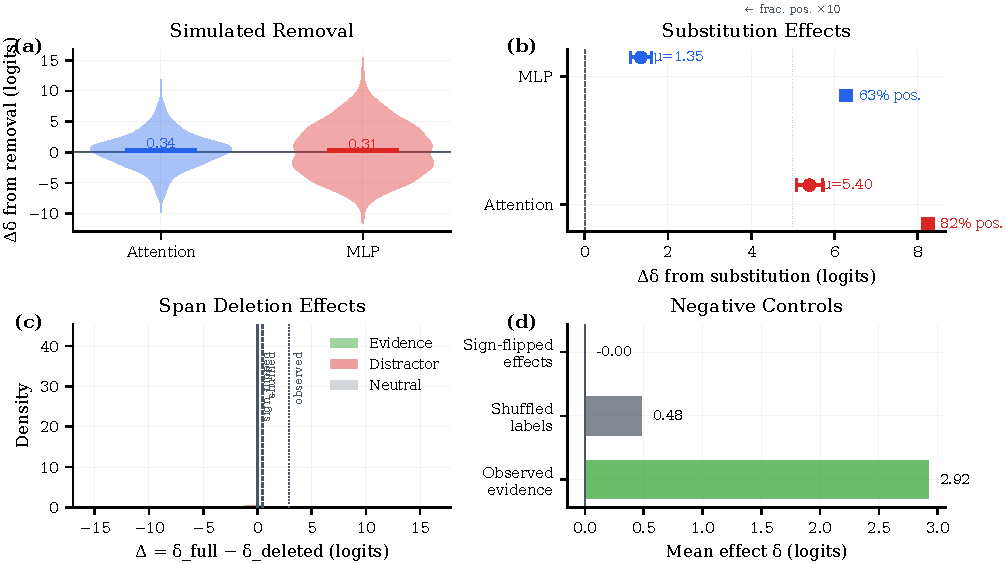
\includegraphics[width=\textwidth]{figures/fig5_counterfactuals.pdf}}
    \caption{Counterfactual validation.
    \textbf{(a)}~Simulated removal by model and component: mean $\Delta\delta$ with bootstrap 95\% CI (logits), vertical zero line.
    \textbf{(b)}~Activation patching distribution for failing trajectories: density of base final margin versus patched final margin, with mean-shift annotation.
    \textbf{(c)}~Substitution summary (remove failing component contribution at target layers, add successful component contribution): mean $\Delta\delta$ with 95\% CI (top) and fraction of positive shifts (bottom).
    \textbf{(d)}~Span deletion causal test: mean deletion effect by operational span label with bootstrap 95\% CI, plus horizontal baselines for observed/shuffled/sign-flipped controls.
    Data: \texttt{ablation\_results.parquet} (3{,}600 rows), \texttt{patching\_results.parquet} (1{,}800 rows), \texttt{span\_labels.parquet} (4{,}200 rows), \texttt{negative\_controls.parquet} (3 rows).}
    \label{fig:causal}
  \end{center}
\end{figure*}

\begin{figure*}[!t]
  \vskip 0.1in
  \begin{center}
    \centerline{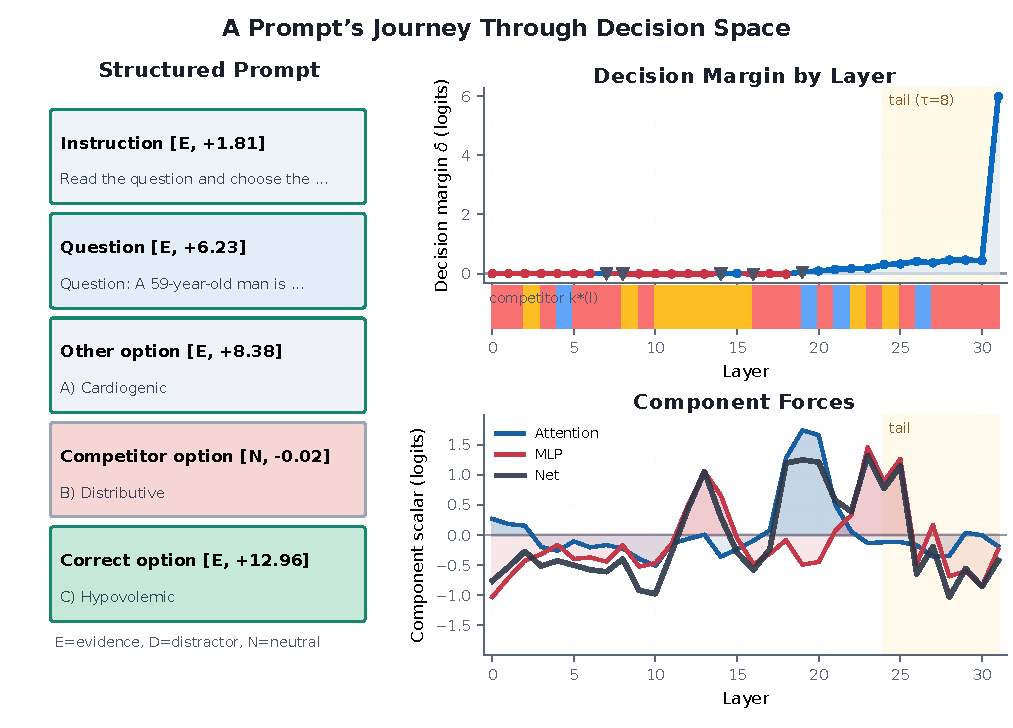
\includegraphics[width=\textwidth]{figures/fig6_prompt_journey.pdf}}
    \caption{A single prompt's journey through decision space (stable-correct trajectory).
    \textbf{(a)}~Structured prompt spans with role fills and operational labels (evidence/distractor/neutral), each annotated with deletion effect~$\Delta$.
    \textbf{(b)}~Decision margin $\delta(l)$ versus real layer index; tail window ($\tau{=}8$, last 8 layers) shaded; per-layer closest-competitor identity shown as a colour strip below the axis; sign flips marked with~$\blacktriangledown$.
    \textbf{(c)}~Component forces: attention scalar $s_{\mathrm{attn}}(l)$ and MLP scalar $s_{\mathrm{mlp}}(l)$ versus layer on the same axis, with positive/negative regions lightly shaded; tail window shaded as in~(b).
    Data: \texttt{decision\_metrics.parquet}, \texttt{tracing\_scalars.parquet}, \texttt{span\_labels.parquet}.}
    \label{fig:flow}
  \end{center}
\end{figure*}



\begin{figure*}[!t]
  \vskip 0.1in
  \begin{center}
    \centerline{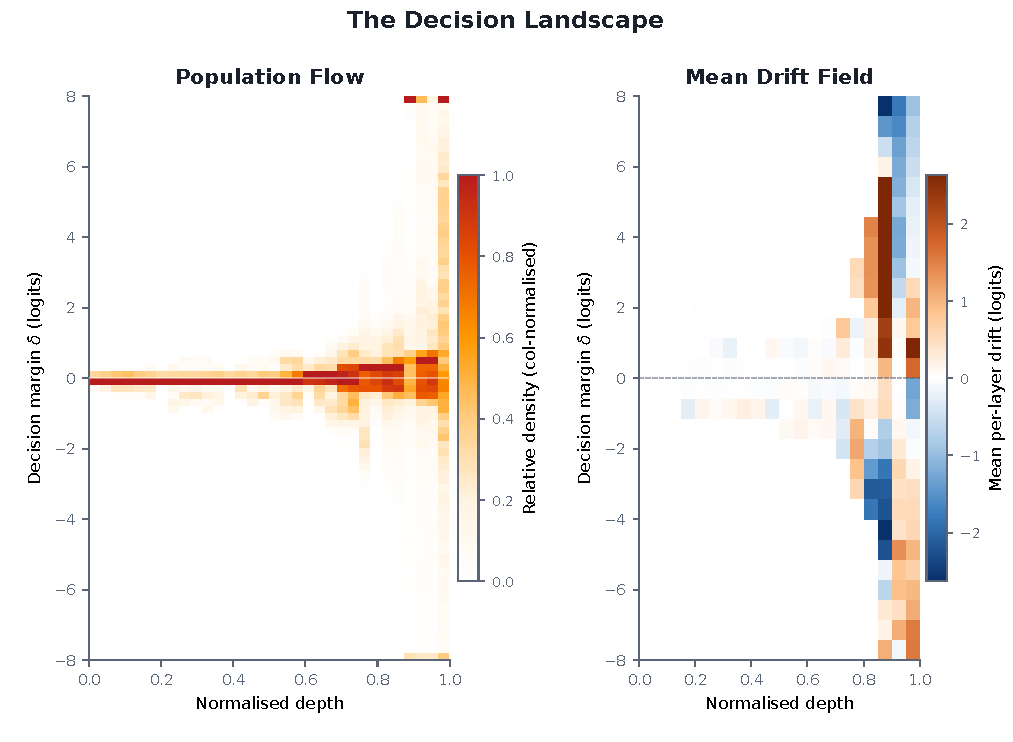
\includegraphics[width=\textwidth]{figures/fig7_decision_landscape.pdf}}
    \caption{The Decision Landscape: all 276,000 (model, prompt, layer) observations projected onto the (normalised depth, $\delta$) plane.
    \textbf{(a)}~\emph{Population Flow.}  Two-dimensional histogram over depth and $\delta$, with \emph{column-wise normalization}: each depth slice is scaled by its own maximum count, so colour encodes relative density within that depth bin (0--1).  Depth and margin bins are coarsened for readability in late layers.
    \textbf{(b)}~\emph{Mean Drift Field.}  Grid over depth and clipped margin ($\delta \in [-8,8]$); each populated cell shows mean per-layer drift $\bar{g}$, with cells of count $<5$ masked to suppress noisy outliers.  Colours use a zero-centred diverging scale (blue: $\bar{g}>0$, red: $\bar{g}<0$).
    Data: \texttt{decision\_metrics.parquet}.}
    \label{fig:landscape}
  \end{center}
\end{figure*}


%% ============================================================
%% 9. DISCUSSION
%% ============================================================
\section{Discussion}
\label{sec:discussion}

\paragraph{Code.}  Repository: \url{https://github.com/gut-puncture/The-Shape-of-Wisdom}.

\textbf{What the primitives buy.}  Rather than ``the model got it wrong,'' we can say ``the model entered the correct region at layer~12 but was pushed out by MLP injection at layer~23.''  This localizes failure, identifies the responsible component, and suggests targeted interventions.

\textbf{Implications for training.}  We refrain from strong claims but note a hypothesis: training procedures that penalize drift disagreement between attention and MLP in late layers might reduce stable-wrong rates.

\textbf{Limitations.}
\vspace{-0.5em}
\begin{enumerate}\setlength{\itemsep}{0pt}
\item \textbf{Restricted four-choice readout.}  Token-bucket scoring over $\{$A, B, C, D$\}$ only; the full vocabulary and hidden-state structure remain invisible.  The model may ``know'' the answer in a representation that our four-token probe cannot detect.
\item \textbf{Linearized counterfactual simulation.}  The drift-bookkeeping model (\cref{alg:removal,alg:substitution}) assumes no downstream adaptation after component modification.  This linearity assumption has not been independently verified; true activation patching with full forward-pass re-inference would provide stronger evidence.
\item \textbf{Threshold conventions.}  $\tau = 8$, $b_{\min} = 0.3$, and zero flips \emph{define} rather than \emph{discover} trajectory-type boundaries.  These thresholds are pre-registered conventions that shift smoothly under perturbation; there is no natural discontinuity.
\item \textbf{Proxy components.}  The margin-aligned projections $s_{\mathrm{attn}}$ and $s_{\mathrm{mlp}}$ discard information orthogonal to the decision direction $d$.  The two-force decomposition captures the signal relevant to the four-choice margin but leaves substantial variance unexplained ($R^2 \leq 0.70$ implies ${\geq}30\%$ residual).
\item \textbf{Circular span labeling.}  Evidence/distractor labels are defined by counterfactual effect on $\delta$, so their separation by $\Delta$ is tautological.  Validation relies on independent signals (attention routing, negative controls).
\item \textbf{Scale.}  Only 7--8B models studied.
\item \textbf{Prompt format.}  Only four-choice MC; open-ended generation may differ.
\item \textbf{Single run.}  Results from one deterministic run (seed 12345).
\end{enumerate}


%% ============================================================
%% 10. RELATED WORK
%% ============================================================
\section{Related Work}

\textbf{Logit lens and tuned lens.}  \citet{nostalgebraist2020} and \citet{belrose2023} project intermediate representations through the unembedding matrix.  We analyze the \emph{trajectory} of projections across layers in the answer-token subspace.

\textbf{Mechanistic interpretability.}  The circuits paradigm~\cite{elhage2021,olsson2022,conmy2023} identifies computational subgraphs.  We characterize trajectory-level dynamics, trading microscopic precision for macroscopic coverage.

\textbf{Probing classifiers.}  Linear probes~\cite{belinkov2022,hewitt2019} test whether representations encode specific properties.  Our $\delta(l)$ is a targeted probe without learned-classifier ambiguity.

\textbf{Causal tracing.}  \citet{meng2022} localize factual associations.  Our span-deletion tests operate at the prompt level; ablations target component types rather than individual positions.

\textbf{Decision dynamics.}  Recent work~\cite{din2023,geva2023} studies layerwise prediction evolution.  We contribute a unified framework connecting descriptive dynamics, mechanistic decomposition, and counterfactual accounting.


%% ============================================================
%% 11. CONCLUSION
%% ============================================================
\section{Conclusion}

A transformer's decision on a multiple-choice question is not a point but a trajectory.  Three measurable quantities---the logit margin $\delta$, its per-layer drift $g$, and the boundary distance $|\delta|$---suffice to classify this trajectory into four outcome types, producing a phase diagram that replicates across architectures and domains.

Decomposing drift into attention and MLP contributions reveals that attention is the sustained positive force across mid-layers for correct answers, while MLP provides a brief supportive burst at depth $0.7$--$0.8$ within an otherwise opposing signal.  For wrong answers, both forces reinforce the incorrect basin.  Counterfactual accounting experiments---both linearized estimates and true input-level span deletions---confirm directionally consistent effects, with MLP substitution producing a 4$\times$ larger mean shift than attention substitution.

The framework is deliberately modest: we claim sufficiency for classification, not necessity; counterfactual relevance under linearity assumptions, not sole causation; and insight from a restricted-choice logit-margin space, not complete representation coverage.  The phase diagram is a map.  The two-force decomposition is a compass.  Together, they provide a vocabulary for navigating the space between a prompt and an answer.


%% ============================================================
%% IMPACT STATEMENT
%% ============================================================
\section*{Impact Statement}

This paper presents work whose goal is to advance the field of mechanistic interpretability by providing diagnostic tools for understanding transformer decision-making.  Improved understanding of model failures may contribute to safer and more reliable AI systems.  We do not foresee specific negative societal consequences beyond those generally associated with advances in machine learning.


%% ============================================================
%% REFERENCES
%% ============================================================
\balance
\bibliography{references}
\bibliographystyle{plainnat}


%% ============================================================
%% APPENDIX
%% ============================================================
\clearpage
\appendix

\section{Threshold Sensitivity Analysis}
\label{sec:appendix_sensitivity}

We vary the trajectory classification parameters and verify that the four-cluster structure persists.

\textbf{Tail length $\tau \in \{6, 8, 10\}$:}  Shorter tails classify more trajectories as stable; longer tails classify more as unstable.  Phase geometry is preserved.

\textbf{Minimum boundary $b_{\min} \in \{0.1, 0.3, 0.5\}$:}  Lower thresholds admit near-boundary trajectories as stable; higher thresholds reclassify them.  Separation degrades gracefully.

\textbf{Late flip threshold $\in \{0, 1\}$:}  Allowing one flip expands the stable class modestly for $\tau = 8$.

\section{Probability-Space Comparison}
\label{sec:appendix_prob}

Replicating the phase diagram using probability margins ($p_c - p_{k^*}$) in place of logit margins produces visible but less separated clusters.  High-confidence decisions compress into a narrow probability range, reducing discrimination.  We recommend logit-space analysis for trajectory work.

\section{PCA Visualizations of Hidden States}
\label{sec:appendix_pca}

PCA on full hidden-state vectors at selected layers shows partially separable trajectory-type clusters in PC1--PC2 space.  However, explained variance is below 15\% for PC1, making these visualizations illustrative rather than evidentiary.

\section{Decomposition Residual Analysis}

The residual $\varepsilon$ from \cref{eq:decomposition} has mean near zero with modest layer-dependent heteroscedasticity (larger variance at layers 12--18).  No systematic bias invalidates the linear approximation.

\section{Per-Domain Breakdowns}

STEM domains show higher stable-wrong rates (confident factual errors).  Humanities show higher instability (ambiguous or context-dependent questions).  Social sciences are intermediate.

\section{Token-Bucket Readout Details}
\label{sec:appendix_buckets}

For each answer letter $L \in \{\mathrm{A}, \mathrm{B}, \mathrm{C}, \mathrm{D}\}$, we construct a token bucket from six variant templates:
\begin{center}
\texttt{"\{L\}"},\; \texttt{" \{L\}"},\; \texttt{"\textbackslash n\{L\}"},\; \texttt{"(\{L\})"},\; \texttt{"\{L\}."},\; \texttt{"\{L\}:"}
\end{center}
Each template string is normalized as follows: (i)~Unicode NFKC normalization, (ii)~strip leading/trailing whitespace, (iii)~uppercase, (iv)~remove surrounding punctuation.  The resulting strings are tokenized with the model's tokenizer to obtain one or more token IDs per template.  The union of all token IDs for letter $L$ forms $\mathrm{bucket}(L)$.

Disjointness is enforced before any analysis: if $\mathrm{bucket}(L_1) \cap \mathrm{bucket}(L_2) \neq \emptyset$ for any $L_1 \neq L_2$, the pipeline halts.  In practice, all three tokenizers in this study produce disjoint buckets.

The max-over-bucket scoring (\cref{eq:bucket}) ensures the readout captures the strongest signal for each letter regardless of how the tokenizer segments the surrounding context.

\section{Tracing-Readout Proxy Validation}
\label{sec:appendix_proxy}

Baseline trajectory metrics use token-bucket scoring (\cref{eq:bucket}).  Decomposition scalars $s_{\mathrm{attn}}(l)$ and $s_{\mathrm{mlp}}(l)$ are computed in the tracing pipeline using canonical single-token option labels (\texttt{A}/\texttt{B}/\texttt{C}/\texttt{D}), not token buckets.  We validate this proxy relationship on the tracing subset by joining \texttt{decision\_metrics.parquet} and \texttt{tracing\_scalars.parquet} on $(\mathrm{model},\mathrm{prompt},\mathrm{layer})$, yielding 55{,}200 (prompt, layer) pairs.

The Pearson correlation between $\delta_{\mathrm{bucket}}(l)$ and $\delta_{\mathrm{single}}(l)$ is $r = 0.55$; the sign-agreement rate is $75.4\%$.  These values indicate a moderate, imperfect proxy.  Decomposition claims should be understood as applying to the single-token tracing readout: directional conclusions (which component steers toward the correct answer) hold for the majority of (prompt, layer) pairs but are not guaranteed to transfer to every bucket-readout example.

\section{Methods}
\label{sec:methods}

\textbf{Metric computation.}  For each prompt~$\times$~model pair, layerwise candidate logits for the four answer-token buckets are extracted from every transformer block.  Scores are computed as max-over-bucket (\cref{eq:bucket}).  $\delta(l)$, $g(l)$, $b(l)$, and $k^*(l)$ are computed per \cref{sec:primitives}.  Probabilities are softmax-normalized over four candidate bucket scores; entropy is $H(l) = -\!\sum_c p_c(l)\log p_c(l)$ with clipping at $10^{-12}$.

\textbf{Layer indexing.}  Models in this study have different layer counts (Qwen: 28, Llama: 32, Mistral: 32).  Cross-model figures use \emph{normalized depth} $l/(L{-}1) \in [0,1]$ to enable comparison.

\textbf{Trajectory classification.}  Sign flips are computed on the sign sequence of $\delta$, ignoring zeros.  Late flips are restricted to the tail window.  Stability requires zero late flips and $\min_{l\, \in\, \mathrm{tail}} b(l) \geq 0.3$.

\textbf{Span parsing.}  Prompt spans are identified via regular-expression boundary detection.  Option spans are re-indexed relative to correctness (\texttt{option\_correct}, \texttt{option\_competitor}, \texttt{option\_other}).  Span effects are computed by deletion and re-inference (true input-level intervention).  Evidence/distractor labels are an \emph{operational definition} using symmetric thresholds at $\pm 0.05$; separation by $\Delta$ is tautological.  Paraphrase stability is assessed on 50 prompts per model.

\textbf{Tracing and decomposition.}  For the tracing subset, attention and MLP outputs are captured via forward hooks using eager attention.  Component scalars are computed as margin change (\cref{eq:s_attn,eq:s_mlp}), equivalent to the dot product with the decision direction (\cref{eq:attn_dot}).  OLS fit uses a 70/30 train/test split at the prompt level with $R^2 \geq 0.70$ enforced.  We validate the proxy relationship between tracing and bucket readouts on the tracing subset: Pearson $r = 0.55$, sign agreement $= 75.4\%$ (\cref{sec:appendix_proxy}); decomposition claims should be read as applying to the single-token tracing readout, which agrees in direction with the bucket readout for approximately three-quarters of (prompt, layer) pairs.

\textbf{Counterfactual experiments.}  Simulated component removal follows \cref{alg:removal} at layers $T = \{20, \ldots, 27\}$; this is a linearized estimate, not a forward-pass intervention.  Simulated substitution follows \cref{alg:substitution}.  Span deletion actually removes spans and re-runs inference.  Negative controls: label-shuffle (256 permutations) and sign-flip (256 iterations).

\textbf{Statistics.}  Bootstrap CIs use 2{,}000 resamples.  Permutation tests use 5{,}000 permutations.  Multiple-comparison correction uses Benjamini--Hochberg with $\alpha = 0.05$.  All random operations use deterministic seeds.

\textbf{Reproducibility.}  The full pipeline runs from a single orchestrator with fail-closed gating.  Intermediate artifacts are persisted as Parquet files with SHA-256 manifests.  Thermal management enforces checkpoint/resume determinism.

\end{document}
